% -*- latex -*-
%%%%%%%%%%%%%%%%%%%%%%%%%%%%%%%%%%%%%%%%%%%%%%%%%%%%%%%%%%%%%%%%
%%%%%%%%%%%%%%%%%%%%%%%%%%%%%%%%%%%%%%%%%%%%%%%%%%%%%%%%%%%%%%%%
%%%%
%%%% This text file is part of the source of 
%%%% `Parallel Computing'
%%%% by Victor Eijkhout, copyright 2012/3/4/5
%%%%
%%%%%%%%%%%%%%%%%%%%%%%%%%%%%%%%%%%%%%%%%%%%%%%%%%%%%%%%%%%%%%%%
%%%%%%%%%%%%%%%%%%%%%%%%%%%%%%%%%%%%%%%%%%%%%%%%%%%%%%%%%%%%%%%%

\Level 0 {Working with global information}
\commandidiom{collective}
\index{collectives|(}

If all processes have individual data, for instance the result
of a local computation, you may want to bring that information
together, for instance to find the maximal computed value
or the sum of all values. Conversely, sometimes one processor has
information that needs to be shared with all.
For this sort of operation, MPI
has \indexterm{collectives}.

There are various cases,
\begin{figure}[ht]
  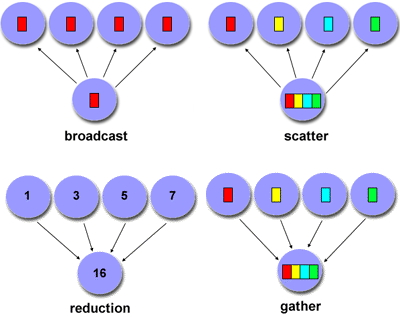
\includegraphics[scale=.8]{collective_comm}  
  \caption{The four most common collectives}
  \label{fig:collectives}
\end{figure}
the most common ones are illustrated in figure~\ref{fig:collectives}.

Above, you saw how each process can perform its own computation
with its own result. You may want to summarize these results
on one process, known as the \indexterm{root process},
for instance to print them out.
If you perform an operation on the data from the processors,
for instance to compute the maximum value, this is known
as a \indexterm{reduction} (section~\ref{sec:bcast}).
On the other hand, if you need to collect and preserve
all computation results, the operation is known
as a \indexterm{gather} (section~\ref{sec:gatherscatter}).

Conversely, one process can have data that needs to be
spread to all others, for instance because it reads it from file.
If the same item needs to be sent to all processes, this
is known as \indexterm{broadcast}.
If the root process sends individual data to each process,
it is called a \indexterm{scatter}.

\begin{exercise}
  \label{ex:collective-cases}
  How would you realize the following scenarios with MPI collectives?
  \begin{itemize}
  \item Let each process compute a random number. You want to print the
    maximum of these numbers to your screen.
  \item Each process computes a random number again. Now you want to
    scale these numbers by their maximum. 
  \item Let each process compute a random number. You want to print on what processor the
    maximum value is computed. 
  \end{itemize}
\end{exercise}

There are more collectives or variants on the above.
\begin{itemize}
\item If you want to gather or scatter information, but the contribution
  of each processor is of a different size, there are `variable' collectives;
  they have a~\n{v} in the name (section~\ref{sec:v-collective}).
\item Sometimes you want a reduction with partial results, where each processor
  computes the sum (or other operation) on the values of lower-numbered processors.
  For this, you use a \indexterm{scan} collective (section~\ref{sec:scan}).
\item If every processor needs to broadcast to every other, you use an
  \indexterm{all-to-all} operation (section~\ref{sec:allreduce}).
\item A barrier is an operation that makes all processes wait until every
  process has reached the barrier (section~\ref{sec:barrier}).
\end{itemize}

Finally, there are some advanced topics in collectives.
\begin{itemize}
\item Non-blocking collectives; section~\ref{sec:mpi3collect}.
\item User-defined reduction operators; section~\ref{sec:mpi:op-create}.
\end{itemize}

\index{collectives|)}

%\input chapters/mpi-intro-collective
\Level 0 {Collectives}
\commandref{collective}

Collectives are operations that involve all processes in a
communicator. (See section~\ref{sec:collective} for an informal listing.)
A~collective is a
single call, and it blocks on all processors.
That does not mean that
all processors exit the call at the same time: because of
implementational details and network
latency they need not be synchronized in their execution.
However, semantically we can say that
a~process can not finish
a collective until every other process has at least started the collective.

In addition to these collective operations, there are operations that
are said to be `collective on their communicator', but which do not
involve data movement. Collective then means that all processors must
call this routine; not to do so is an error that will 
manifest itself in `hanging' code. One such example is
\n{MPI_Win_fence}.

\Level 1 {Rooted collectives: broadcast, reduce}
\commandref{bcast}

One simple collective is the broadcast, where one process has some
data that needs to be shared with all others. One scenario is that
processor zero can parse the commandline arguments of the executable
and send the values to all other processors.
Another scenario is that you want one processor to read data from file
and send it to the other processors: that is likely to be more efficient
than having every process open the file.

The broadcast call has the following structure:
\begin{verbatim}
MPI_Bcast( data..., root , comm);
\end{verbatim}
The root is the process that is sending its data.
Typically, it will be the root of a broadcast tree.
The \n{comm} argument is a communicator:
for now you can use \n{MPI_COMM_WORLD}.
Unlike with send/receive there is no message tag,
because collectives are blocking, so you can have only one active at a
time. 

The data in a broadcast (or any other MPI operation for that matter)
is specified as
\begin{itemize}
\item A buffer. In~C this is the address in memory of the data. This means
  that you broadcast a single scalar as \n{MPI_Bcast( &value, ... )},
  but an array as \n{MPI_Bcast( array, ... )}.
\item The number of items and their datatype. The allowable datatypes
  are such things as \n{MPI_INT} and \n{MPI_FLOAT} for~C, and
  \n{MPI_INTEGER} and \n{MPI_REAL} for Fortran, or more complicated types.
  See section~\ref{ref:mpidata} for details.
\end{itemize}
\begin{pythonnote}
  In python it is both possible to send objects, and to send
  more C-like buffers. The two possibilities correspond to
  different routine names; the buffers have to be created as \n{numpy}
  objects.
\end{pythonnote}

\begin{exercise}
  \label{ex:argv-bcast}
  If you give a commandline argument to a program, that argument is available
  as a character string as part of the \n{argv,argc} pair that you typically use
  as the arguments to your main program. You can use the function \n{atoi} to
  convert such a string to integer.

  Write a program where process~0 looks for an integer on the commandline, and
  broadcasts it to the other processes. Initialize the buffer on all processes, and
  let all processes print out the broadcast number,
  just to check that you solved the problem correctly.
\end{exercise}

The reverse of a broadcast is a reduction:
\begin{verbatim}
MPI_Reduce( senddata, recvdata..., operator,
    root, comm ); 
\end{verbatim}
Now there is a separate buffer for outgoing data, on all processors,
and incoming data, only relevant on the root. Also, you have to
indicate how the data is to be combined. Popular choices are
\indexmpishow{MPI_SUM}, \indexmpishow{MPI_PROD} and
\indexmpishow{MPI_MAX}, but complicated operators such as finding the
location of the maximum value exist. You can also define your own
operators; section~\ref{ref:mpi:op-create}.

\begin{exercise}
  \label{ex:randommax}
  Write a program where each process computes a random number, and process~0
  finds and prints the maximum generated value. Let each process print its value,
  just to check the correctness of your program.

\end{exercise}

  Here is how you initialize the random number generator uniquely on each process:

{\footnotesize
\begin{verbatim}
C:

// Initialize the random number generator
srand((int)(mytid*(double)RAND_MAX/ntids));
// compute a random number
randomfraction = (rand() / (double)RAND_MAX);
\end{verbatim}
\begin{verbatim}
Fortran:

  integer :: randsize
  integer,allocatable,dimension(:) :: randseed
  real :: random_value

  call random_seed(size=randsize)
  allocate(randseed(randsize))
  do i=1,randsize
     randseed(i) = 1023*mytid
  end do
  call random_seed(put=randseed)
\end{verbatim}
}

Collective operations can also take an array argument, instead of just a scalar.
In that case, the operation is applied pointwise to each location in the array.

\begin{exercise}
  \label{ex:randomcoord}
  Create on each process an array of length~2 integers, and put the values $1,2$
  in it on each process. Do a sum reduction on that array. Can you predict what the result should be?
  Code it. Was your prediction right?
\end{exercise}

\Level 1 {Rooted collectives: gather and scatter}
\commandref{gatherscatter}

In the \indexmpishow{MPI_Scatter} operation, the root spreads information to
all other processes. The difference with a broadcast is that it involves
individual information from/to every process. Thus, the gather operation typically 
has an array of items, one coming from each sending process, and scatter has an array,
\begin{figure}[ht]
  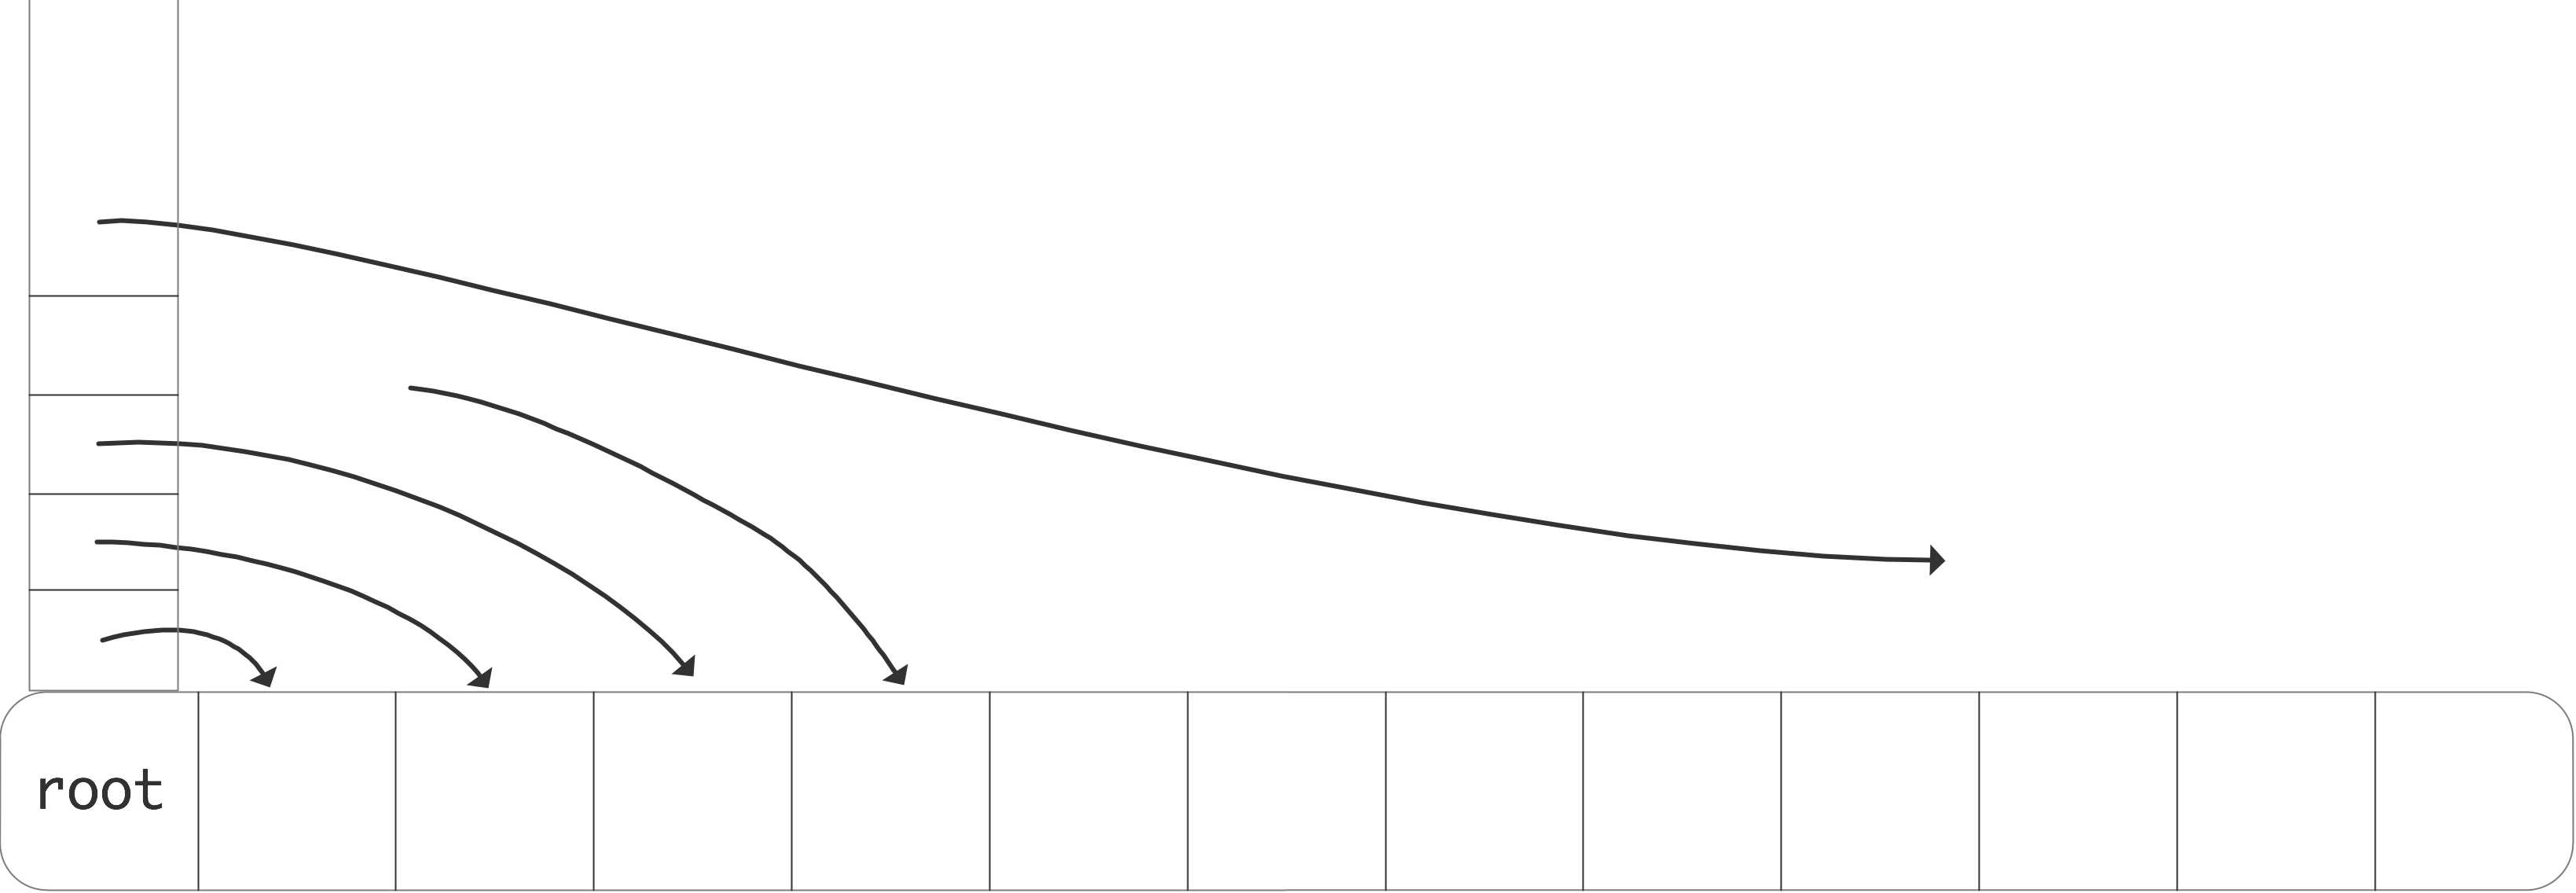
\includegraphics[scale=.12]{graphics/scatter-simple}
  \caption{A scatter operation}
  \label{fig:scatter}
\end{figure}
with an individual item for each receiving process; see figure~\ref{fig:scatter}.

These gather and scatter collectives have a different parameter list from
the broadcast/reduce. The broadcast/reduce involves the same amount
of data on each process, so it was enough to have a buffer, datatype, and size.
In the gather/scatter calls you have
\begin{itemize}
\item a large buffer on the root, with a datatype and size specification, and
\item a smaller buffer on each process, with its own type and size specification.
\end{itemize}
Of course, since we're in SPMD mode, even non-root processes have
the argument for the send buffer, but they ignore it. For instance:
\begin{verbatim}
int MPI_Scatter
  (void* sendbuf, int sendcount, MPI_Datatype sendtype, 
   void* recvbuf, int recvcount, MPI_Datatype recvtype, 
   int root, MPI_Comm comm) 
\end{verbatim}
The \n{sendcount} is not, as you might expect, the total length of the
sendbuffer; instead, it is the amount of data sent to each process.

\begin{exercise}
  \label{ex:randomwhere}
  Let each process compute a random number. You want to print on what processor the
  maximum value is computed. What collective do you use? Write
  a short program.
\end{exercise}

\Level 1 {Variable-size-input collectives}
\commandref{v-collective}

In the gather and scatter call above each processor received or sent
an identical number of items. In many cases this is appropriate, but
sometimes each processor wants or contributes an individual number of
items. 

Let's take the gather calls as an example. Assume that each processor 
does a local computation that produces a number of data elements,
and this number is different for each processor (or at least not
the same for all). In the regular \n{MPI_Gather} call the root processor
had a buffer of size~$nP$, where $n$~is the number of elements produced
on each processor, and $P$~the number of processors. The contribution
from processor~$p$ would go into locations $pn,\ldots,(p+1)n-1$.

For the variable case, we first need to compute the total required
buffer size. This can be done through a simple \indexmpishow{MPI_Reduce}
with \indexmpishow{MPI_SUM} as reduction operator:
the buffer size is $\sum_p n_p$ where $n_p$~is the number of elements
on processor~$p$. But you can also postpone
this calculation for a minute. 

The next question is where the contributions of the processor will
go into this buffer. For the contribution from processor~$p$
that is $\sum_{q<p}n_p,\ldots\sum_{q\leq p}n_p-1$. To compute this,
the root processor needs to have all the $n_p$ numbers, and it can collect
them with an \indexmpishow{MPI_Gather} call.

We now have all the ingredients.
All the processors specify a send buffer just as with \n{MPI_Gather}.
However, the receive buffer specification on the root is more complicated. 
It now consists of:
\begin{verbatim}
outbuffer, array-of-outcounts, array-of-displacements, outtype
\end{verbatim}
and you have just seen how to construct that information.

\Level 1 {Scan operations}
\commandref{scan}

The \indexmpishow{MPI_Scan} operation also performs a reduction, but it keeps 
the partial results. That is, if processor~$i$ contains a number~$x_i$, 
and $\oplus$ is an operator,
then the scan operation leaves $x_0\oplus\cdots\oplus x_i$ on processor~$i$.
\begin{verbatim}
MPI_Scan( send data, recv data, operator, communicator);
\end{verbatim}
This type of operation is often called a \indexterm{prefix operation};
see \HPSCref{app:prefix}.

The \n{MPI_Scan} routine is an \indextermsub{inclusive}{scan} operation.
Often, the more useful variant is the \indextermsub{exclusive}{scan}
\indexmpishow{MPI_Exscan}
\begin{verbatim}
MPI_Exscan( send data, recv data, operator, communicator);
\end{verbatim}
with the same prototype. 

\begin{exercise}
  The exclusive definition, which computes
  $x_0\oplus x_{i-1}$ on processor~$i$, can easily be derived
  from the inclusive operation for operations such as \n{MPI_PLUS} or \n{MPI_MULT}.
  Are there operators where that is not the case?
\end{exercise}

The \n{MPI_Scan} operation is often useful with indexing data. Suppose that
every processor~$p$ has a local vector where the number of elements~$n_p$ is dynamically 
determined. In order to translate the local numbering $0\ldots n_p-1$ to a global numbering
one does a scan with the number of local elements as input. The output is then the global 
number of the first local variable.

\begin{exercise}
  Do you use \n{MPI_Scan} or \n{MPI_Exscan} for this operation? How
  would you describe the result of the other scan operation, given the
  same input?
\end{exercise}

It is possible to do a \indexterm{segmented scan}. Let $x_i$ be a series of numbers
that we want to sum to $X_i$ as follows. Let $y_i$ be a series of booleans such that
\[ 
\begin{cases}
  X_i=x_i&\hbox{if $y_i=0$}\\
  X_i=X_{i-1}+x_i&\hbox{if $y_i=1$}
\end{cases}
\]
(This is the basis for the implementation of the \indexterm{sparse matrix vector product}
as prefix operation; see \HPSCref{sec:spmvp-prefix}.)
This means that $X_i$ sums the segments between locations where $y_i=0$ and the
first subsequent place where $y_i=1$. To implement this, you need a user-defined operator
\[ 
\begin{pmatrix}  X\\ x\\ y\end{pmatrix}
=
\begin{pmatrix}  X_1\\ x_1\\ y_1\end{pmatrix}
\bigoplus
\begin{pmatrix}  X_2\\ x_2\\ y_2\end{pmatrix}\colon
  \begin{cases}
    X=x_1+x_2&\hbox{if $y_2==1$}\\ X=x_2&\hbox{if $y_2==0$}
  \end{cases}
\]
This operator is not communitative, and it needs to be declared as such
with \indexmpishow{MPI_Op_create}; see section~\ref{ref:mpi:op-create}

\Level 1 {User-defined reductions}
\commandref{mpi:op-create}

For use in reductions and scans it is possible to define your own operator.

\Level 1 {Reduce-scatter}
\commandref{reducescatter}

There are several MPI collectives that are functionally equivalent to
a combination of others. You have already seen \n{MPI_Allreduce} which
is equivalent to a reduction followed by a broadcast. Often such
combinations can be more efficient than using the individual calls;
see~\HPSCref{sec:collective}.

Here is another example: \indexmpishow{MPI_Reduce_scatter} is equivalent
to a reduction on an array of data (meaning a pointwise reduction on each
array location) followed by a scatter of this array to the individual 
processes.

One important example of this command is the
\indextermsub{sparse}{matrix-vector product};
see~\HPSCref{sec:spmvp-performance} for background information.
Each process contains one or more matrix rows, so by looking at indices
the process can decide what other processes it needs data from.
The problem is for a process to find out what other processes 
it needs to send data to. 

Using \indexmpishow{MPI_Reduce_scatter} the process goes as follows:
\begin{itemize}
\item Each process creates an array of ones and zeros, describing who
  it needs data from.
\item The reduce part of the reduce-scatter yields an array of
  requester counts; after the scatter each process knows how many
  processes request data from it.
\item Next, the sender processes need to find out what elements are
  requested from it. For this, each process sends out arrays of
  indices.
\item The big trick is that each process now knows how many of these
  requests will be coming in, so it can post precisely that many
  \n{MPI_Irecv} calls, with a source of \indexmpishow{MPI_ANY_SOURCE}.
\end{itemize}

\Level 1 {`All'-type collectives}
\commandref{allreduce}

In many applications the result of a collective is needed on all processes.
For instance, if $x,y$ are distributed vector objects, and you want to compute
\[ y- (x^ty)x \]
you need the inner product value on all processors. You could do this
by writing a reduction followed by a broadcast, but more efficient
algorithms exist.  Surprisingly, an `all-gather' operation takes as
long as a rooted gather (see~\HPSCref{sec:collective} for details).

Thus, MPI has the following operations:
\begin{itemize}
\item \indexmpishow{MPI_Allreduce} is equivalent to a \indexmpishow{MPI_Reduce} followed by a broadcast.
\item \indexmpishow{MPI_Allgather} is equivalent to a \indexmpishow{MPI_Gather} followed by a broadcast.
\item \indexmpishow{MPI_Allgatherv} is equivalent to an \indexmpishow{MPI_Gatherv} followed by a broadcast.
\item \indexmpishow{MPI_Alltoall}, \indexmpishow{MPI_Alltoallv}.
\end{itemize}

\Level 1 {Non-blocking collectives}
\commandref{mpi3collect}

Above you have seen how the `Isend' and `Irecv' routines can overlap communication
with computation. This is not possible with the collectives you have seen so far:
they act like blocking sends or receives.
However, there are also \indextermsub{non-blocking}{collectives}.
These have roughly the same calling sequence as their blocking counterparts,
except that they output an \indexmpishow{MPI_Request}. You
can then use an \indexmpishow{MPI_Wait} call to make sure the collective
has completed.

Such operations can be used to increase efficiency.
For instance, computing
\[ y \leftarrow Ax + (x^tx)y \]
involves a matrix-vector product, which is dominated by computation
in the \indextermsub{sparse}{matrix} case, and an inner product which is 
typically dominated by the communication cost. You would code this as
\begin{verbatim}
MPI_Iallreduce( .... x ..., &request);
// compute the matrix vector product
MPI_Wait(request);
// do the addition
\end{verbatim}

This can also be used for 3D FFT operations~\cite{Hoefler:case-for-nbc}.
Occasionally, a non-blocking collective can be used for non-obvious purposes,
such as the \indexmpishow{MPI_Ibarrier} in~\cite{Hoefler:2010:SCP}.

\Level 1 {Barrier and all-to-all}
\commandref{barrier}

There are two collectives we have not mentioned yet. A~barrier is a
call that blocks all processes until they have all reached the barrier
call. This call's simplicity is contrasted with its usefulness, which
is very limited. It is almost never necessary to synchronize processes
through a barrier: for most purposes it does not matter if processors
are out of sync. Conversely, collectives (except the new non-blocking
ones) introduce a barrier of sorts themselves.

The all-to-all call is a generalization of a scatter and gather: every
process is scattering an array of data, and every process is gathering
an array of data. There is also a `v' variant of this routine.

\Level 1 {Performance of collectives}

It is easy to visualize a broadcast as in figure~\ref{fig:bcast-simple}:
see figure~\ref{fig:bcast-simple}.
\begin{figure}[ht]
  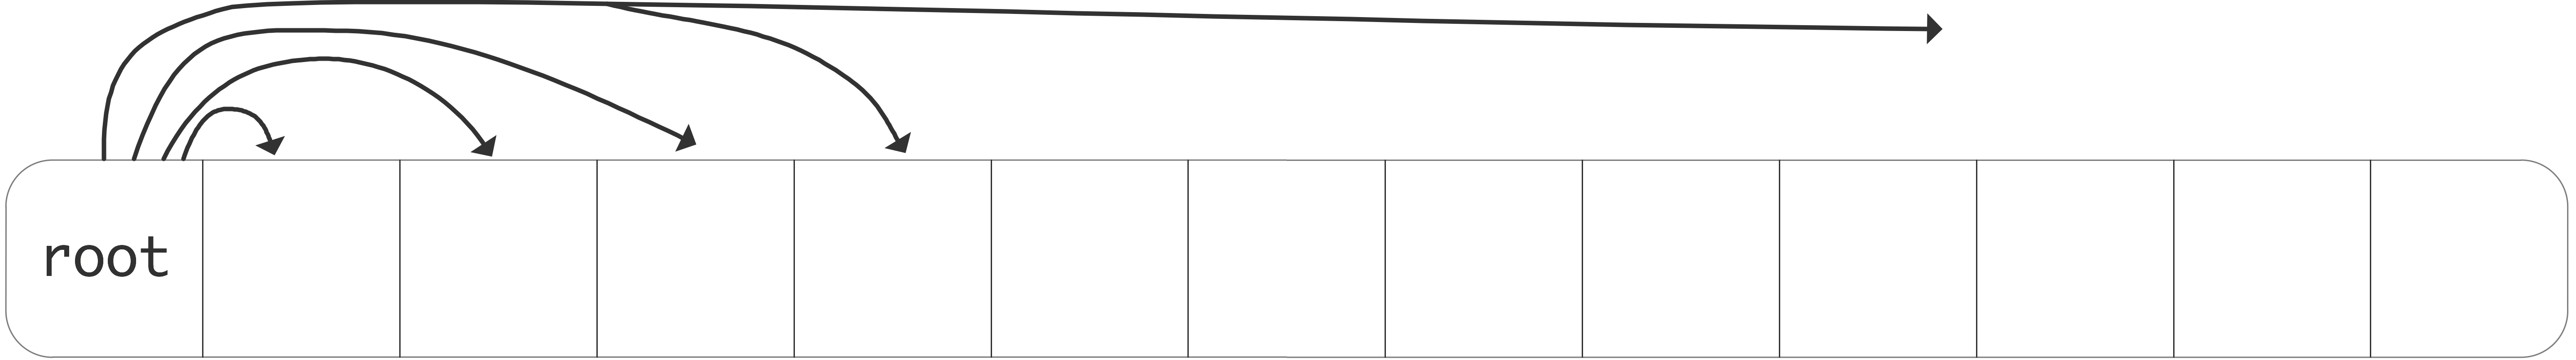
\includegraphics[scale=.08]{graphics/bcast-simple}
  \caption{A simple broadcast}
  \label{fig:bcast-simple}
\end{figure}
the root sends all of its data directly to every other process.
While this describes the semantics of the operation, in practice
the implementation works quite differently.

The time that a message takes can simply be modeled as
\[ \alpha +\beta n, \]
where $\alpha$~is the \indexterm{latency}, a~one time
delay from establishing the communication between two processes,
and $\beta$~is the time-per-byte, or the inverse of the \indexterm{bandwidth},
and $n$~the number of bytes sent.

Under the assumption that
a processor can only send one message at a time,
the broadcast in
figure~\ref{fig:bcast-simple} would take a time proportional to the
number of processors. One way to ameliorate that is to structure the
broadcast in a tree-like fashion.
\begin{figure}[ht]
  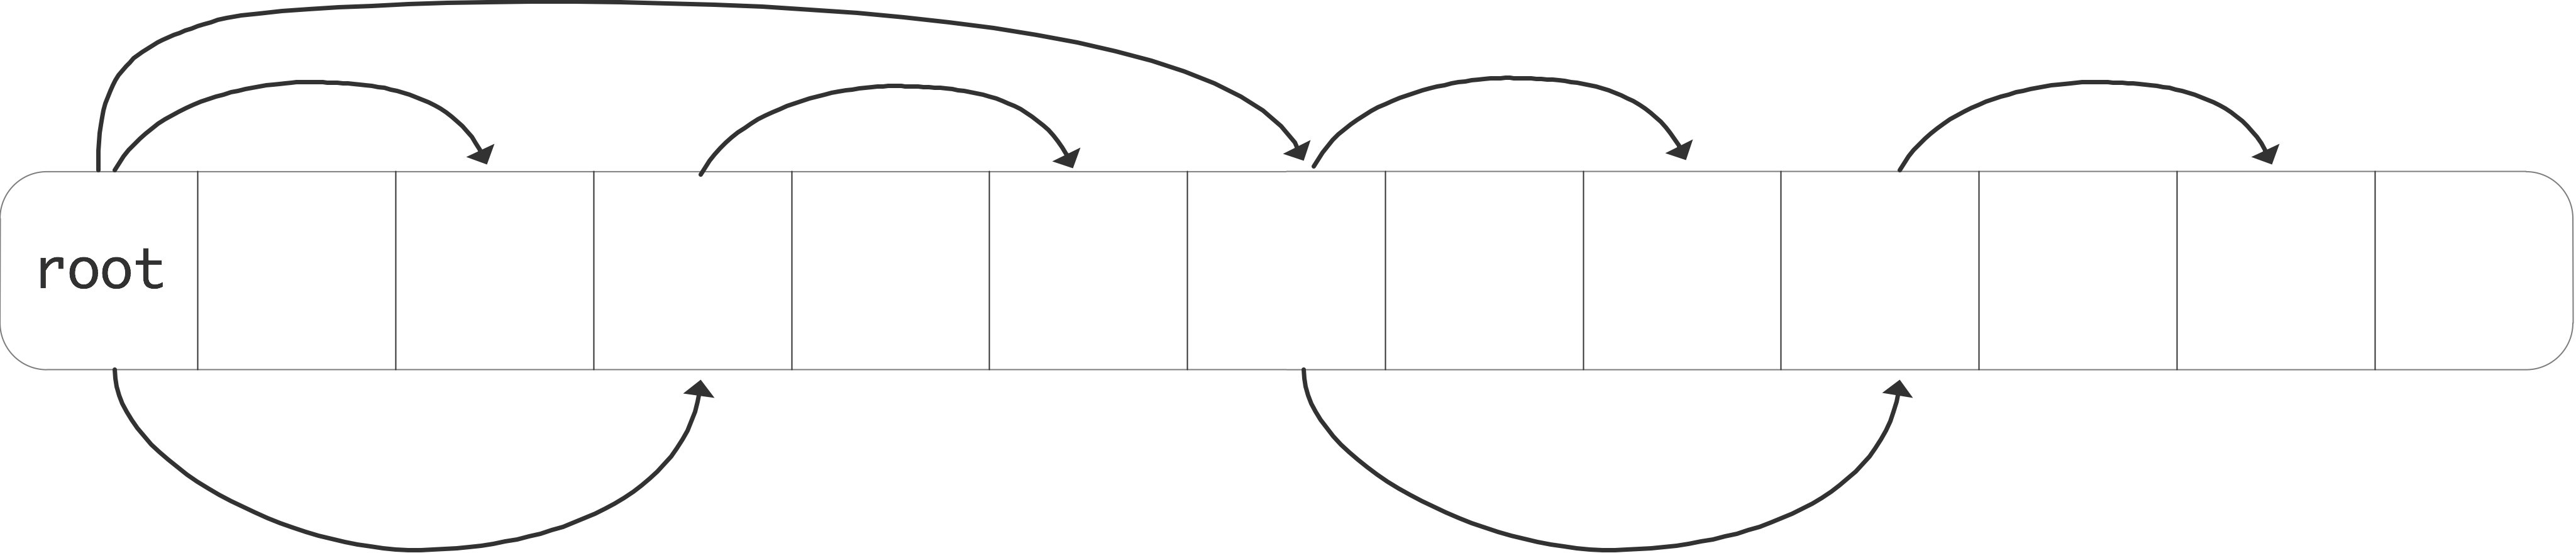
\includegraphics[scale=.1]{graphics/bcast-tree}
  \caption{A tree-based broadcast}
  \label{fig:bcast-tree}
\end{figure}
This is depicted in figure~\ref{fig:bcast-tree}. How does the
communication time now depend on the number of processors? The theory
of the complexity of collectives is described in more detail in
\HPSCref{sec:collective}; see also~\cite{Chan2007Collective}.

\Level 1 {Collectives and synchronization}

Collectives, other than a barrier, have a synchronizing effect between processors.
For instance, in
\begin{verbatim}
MPI_Bcast( ....data... root);
MPI_Send(....);
\end{verbatim}
the send operations on all processors will occur after the root executes
the broadcast. 
\begin{figure}[ht]
  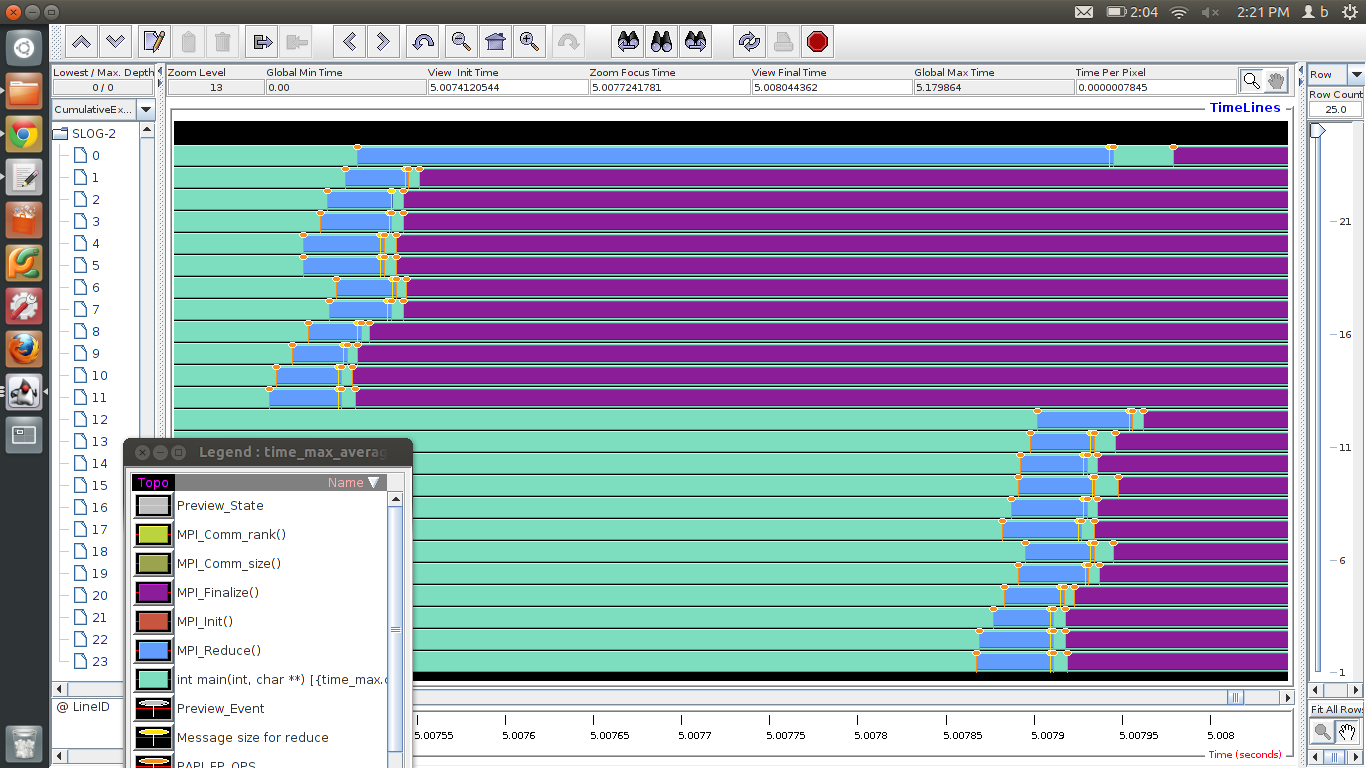
\includegraphics[scale=.35]{graphics/reduce-two-node}
  \caption{Trace of a reduction operation between two dual-socket 12-core nodes}
  \label{fig:trace-reduce}
\end{figure}
Conversely, in a reduce operation the root may have to wait for 
other processors. This is illustrated in figure~\ref{fig:trace-reduce}, which 
gives a TAU trace of
a reduction operation on two nodes, with two six-core sockets (processors) each.
We see that\footnote
{This uses mvapich version 1.6; in version 1.9 the implementation of an on-node reduction
has changed to simulate shared memory.}:
\begin{itemize}
\item In each socket, the reduction is a linear accumulation;
\item on each node, cores zero and six then combine their result;
\item after which the final accumulation is done through the network.
\end{itemize}
We also see that the two nodes are not perfectly in sync, which is normal for MPI
applications. As a result, core~0 on the first node will sit idle until it receives the partial
result from core~12, which is on the second node.

While collectives synchronize in a loose sense, it is not possible to
make any statements about events before and after the collectives
between processors:
\begin{verbatim}
...event 1...
MPI_Bcast(....);
...event 2....
\end{verbatim}
Consider a specific scenario:
\begin{verbatim}
switch(rank) { 
    case 0: 
        MPI_Bcast(buf1, count, type, 0, comm); 
        MPI_Send(buf2, count, type, 1, tag, comm); 
        break; 
    case 1: 
        MPI_Recv(buf2, count, type, MPI_ANY_SOURCE, tag, comm, status); 
        MPI_Bcast(buf1, count, type, 0, comm); 
        MPI_Recv(buf2, count, type, MPI_ANY_SOURCE, tag, comm, status); 
        break; 
    case 2: 
        MPI_Send(buf2, count, type, 1, tag, comm); 
        MPI_Bcast(buf1, count, type, 0, comm); 
        break; 
}
\end{verbatim}
Note the \n{MPI_ANY_SOURCE} parameter in the receive calls on processor~1.
One obvious execution of this would be:
\begin{enumerate}
\item The send from~2 is caught by processor~1;
\item Everyone executes the broadcast;
\item The send from~0 is caught by processor~1.
\end{enumerate}
However, it is equally possible to have this execution:
\begin{enumerate}
\item Processor~0 starts its broadcast, then executes the send;
\item Processor~1's receive catches the data from~0, then it executes
  its part of the broadcast;
\item Processor~1 catches the data sent by~2, and finally processor~2
  does its part of the broadcast.
\end{enumerate}


